\documentclass[10pt,aspectratio=169]{beamer}

% Theme and appearance
\usetheme{Madrid}
\usecolortheme{spruce}
\setbeamertemplate{navigation symbols}{}

% pdfLaTeX-safe font/input setup (ASCII-only paths recommended)
\usepackage[T1]{fontenc}
\usepackage[utf8]{inputenc}
\usepackage{lmodern}

% Math and graphics
\usepackage{amsmath, amssymb, bm}
\usepackage{graphicx}
\graphicspath{{images/}} % Put used PNGs into an Overleaf folder named images/
\usepackage{tikz}
\usetikzlibrary{arrows.meta, positioning}
\usepackage{booktabs}
\usepackage{hyperref}

% Metadata
\title{On-Policy Distillation}
\subtitle{Algorithm Details and Why Reverse KL Divergence}
\author{Prepared by You}
\institute{Study Notes}
\date{\today}

\begin{document}

% Title
\begin{frame}
  \titlepage
\end{frame}

% Motivation (brief)
\begin{frame}{Motivation (brief)}
  \begin{itemize}
    \item Deploying large, high-performing teacher policies can be expensive at inference time.
    \item Distillation trains a smaller student to imitate a strong teacher while preserving performance.
    \item On-policy distillation minimizes distribution shift by training on states induced by the student itself.
    \item Aim: stable imitation that aligns with trusted policy update principles (e.g., trust-region) using KL constraints.
  \end{itemize}
\end{frame}

% Problem setup
\begin{frame}{Setup}
  Consider an MDP $(\mathcal{S}, \mathcal{A}, P, r, \gamma)$.\\[2mm]
  \textbf{Teacher policy}: $\pi_T(a\mid s)$ (fixed).\\
  \textbf{Student policy}: $\pi_S(a\mid s;\,\theta)$ (trainable).\\[2mm]
  Objective (per state $s$ sampled from the student's on-policy distribution):
  \[
    \min_{\theta} \; \mathbb{E}_{s \sim d^{\pi_S}}\big[\, \mathcal{L}(\pi_S(\cdot\mid s),\,\pi_T(\cdot\mid s)) 
    \; + \; \beta\, \mathcal{R}(\pi_S) \,\big]
  \]
  where $\mathcal{L}$ is a divergence between action distributions and $\mathcal{R}$ can include entropy regularization.
\end{frame}

% High-level algorithm flow
\begin{frame}{On-Policy Distillation: High-level Flow}
  \begin{enumerate}
    \item Roll out the \textbf{student} (optionally mixed with the teacher for safety) to collect trajectories $\{s_t\}$.
    \item For each visited state $s$: query the \textbf{teacher} for $\pi_T(\cdot\mid s)$ or action samples.
    \item Minimize a KL-based loss between $\pi_S(\cdot\mid s)$ and $\pi_T(\cdot\mid s)$ on the \textbf{student's} state distribution.
    \item Apply trust-region style control via a KL constraint/penalty to ensure stable updates.
    \item Periodically evaluate; adjust temperature, KL coefficient, or rollout mixing as needed.
  \end{enumerate}
\end{frame}

% Pseudocode
\begin{frame}{Pseudocode}
\small
\begin{block}{On-Policy Distillation}
\begin{enumerate}
  \item Initialize student parameters $\theta$ and fixed teacher $\pi_T$.
  \item \textbf{Repeat} for $k=1,2,\dots$:
  \begin{enumerate}
    \item Collect trajectories by running $\pi_S(\cdot\mid s;\theta)$ (optionally mix with $\pi_T$ with prob. $\alpha$).
    \item For each state $s$ in the batch, obtain $\pi_T(\cdot\mid s)$ (or logits) and compute loss
    \[
      \mathcal{L}_k = \mathbb{E}_{s\sim d^{\pi_S}}\big[\underbrace{\mathrm{KL}(\pi_S\,\Vert\,\pi_T)}_{\text{reverse KL}}\big]
      \; + \; \beta\,\mathbb{E}[\,\mathcal{H}(\pi_S)\,] \; + \; \lambda\,\mathrm{KL}(\pi_S\,\Vert\,\pi_{S,\text{old}})
    \]
    (the last term is optional, acting like a trust-region penalty).
    \item Update $\theta \leftarrow \theta - \eta\,\nabla_\theta \mathcal{L}_k$.
  \end{enumerate}
  \item \textbf{Until} convergence.
\end{enumerate}
\end{block}
\end{frame}

% KL options
\begin{frame}{Forward vs Reverse KL}
  For a fixed state $s$, compare two directions:
  \[\small
    \mathrm{FKL}:\; \mathrm{KL}(\pi_T\,\Vert\,\pi_S) 
    = \sum_a \pi_T(a\mid s)\log\frac{\pi_T(a\mid s)}{\pi_S(a\mid s)}
  \]
  \[\small
    \mathrm{RKL}:\; \mathrm{KL}(\pi_S\,\Vert\,\pi_T) 
    = \sum_a \pi_S(a\mid s)\log\frac{\pi_S(a\mid s)}{\pi_T(a\mid s)}
  \]
  \vspace{1mm}
  \begin{itemize}
    \item \textbf{FKL} (mass-covering): penalizes missing teacher support; tends to spread probability mass.
    \item \textbf{RKL} (mode-seeking): penalizes assigning mass where teacher has little; focuses on teacher's peaks.
  \end{itemize}
\end{frame}

% Intuition figure (TikZ)
\begin{frame}{RKL is mode-seeking; FKL is mass-covering}
\centering
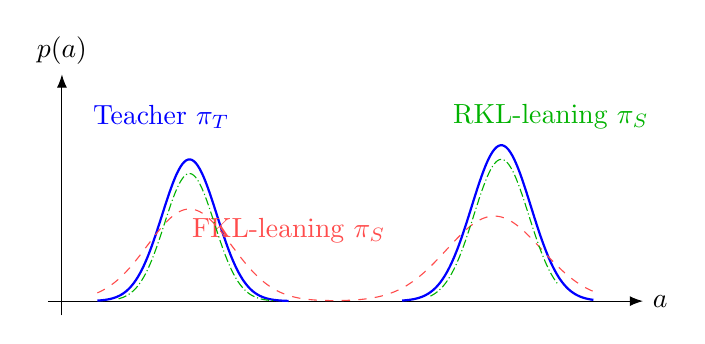
\begin{tikzpicture}[scale=0.9]
  % Axes
  \draw[-{Latex}] (-0.2,0) -- (8.2,0) node[right]{$a$};
  \draw[-{Latex}] (0,-0.2) -- (0,3.2) node[above]{$p(a)$};
  % Teacher modes (two bumps, qualitative)
  \draw[blue, thick, domain=0.5:3.2, samples=100] plot(\x, {2*exp(-((\x-1.8)^2)/0.3)});
  \draw[blue, thick, domain=4.8:7.5, samples=100] plot(\x, {2.2*exp(-((\x-6.2)^2)/0.35)});
  \node[blue] at (1.4,2.6) {Teacher $\pi_T$};
  % Student under FKL (broader mass)
  \draw[red!70, dashed, domain=0.5:7.5, samples=200] plot(\x, {1.3*exp(-((\x-1.8)^2)/0.7) + 1.2*exp(-((\x-6.1)^2)/0.9)});
  \node[red!70] at (3.2,1.0) {FKL-leaning $\pi_S$};
  % Student under RKL (mode-seeking)
  \draw[green!70!black, densely dashdotted, domain=0.8:3.0, samples=100] plot(\x, {1.8*exp(-((\x-1.8)^2)/0.25)});
  \draw[green!70!black, densely dashdotted, domain=5.2:7.0, samples=100] plot(\x, {2.0*exp(-((\x-6.2)^2)/0.3)});
  \node[green!70!black] at (6.9,2.6) {RKL-leaning $\pi_S$};
\end{tikzpicture}
\end{frame}

% Why reverse KL
\begin{frame}{Why use Reverse KL in On-Policy Distillation?}
  \begin{itemize}
    \item \textbf{Stability via trust regions}: RKL aligns with constraints like $\mathrm{KL}(\pi_{\text{old}}\,\Vert\,\pi_{\text{new}})$ from TRPO/PPO-style updates, discouraging unsafe shifts.
    \item \textbf{Mode-seeking imitation}: Forces the student to put mass only where the teacher is confident, reducing risky actions on critical states.
    \item \textbf{On-policy distribution matching}: When states come from $d^{\pi_S}$, RKL punishes assigning high prob. to off-teacher actions actually taken by the student, tightening imitation where it matters.
    \item \textbf{Practical optimization}: Often pairs well with temperature scaling of the teacher and entropy regularization of the student.
  \end{itemize}
\end{frame}

% Image from the KL article (provided asset)
\begin{frame}{Forward vs Reverse KL (visual)}
  \centering
  
\includegraphics[width=0.9\linewidth]{20240112163924.png}
\end{frame}

% Another image if desired
\begin{frame}{Another KL intuition graphic}
  \centering
  
\includegraphics[width=0.9\linewidth]{20240112163931.png}
\end{frame}

% A generic RL image
\begin{frame}{RL context}
  \centering
  
\includegraphics[width=0.7\linewidth]{chess.png}
\end{frame}

% Practical tips
\begin{frame}{Practical Tips}
  \begin{itemize}
    \item \textbf{Rollout mixing}: Start with a small probability $\alpha$ of taking teacher actions to avoid early collapse; anneal $\alpha\to 0$.
    \item \textbf{Temperature}: Soften or sharpen $\pi_T$ logits with temperature $\tau$ for better gradients.
    \item \textbf{Entropy reg.}: Encourage exploration early, then reduce the weight $\beta$.
    \item \textbf{KL control}: Use a target KL with adaptive coefficient $\lambda$; clip or schedule the penalty.
    \item \textbf{Evaluation}: Track success rate/return vs. the teacher; monitor per-state KL and action agreement.
  \end{itemize}
\end{frame}

% Summary
\begin{frame}{Summary}
  \begin{itemize}
    \item On-policy distillation trains on the student's own state distribution, reducing covariate shift vs. pure offline cloning.
    \item Reverse KL is a natural, mode-seeking and stability-friendly choice for policy imitation under trust-region style control.
    \item Combine with rollout mixing, temperature scaling, and entropy regularization for robust practice.
  \end{itemize}
\end{frame}

\end{document}
